We now want to show that this algorithm takes logarithmically many steps in expectation. We will look at the edges of the graph. We remove edges if they are incident to vertices that stop. We'll show that in expectation half the edges are removed in every round. 

Let $G_i=(V_i,E_i)$ be the graph at the beginning of the $i$th round. Obviously this is a random graph, as it results from a random process. Let $X_i$ be the random variable indicating the number of removed edges in phase $i$.

\begin{lem} \label{lem:at_least_half}$\E(X_i |G_i = G) \geq |E(G)|/2$ \end{lem}

%todo elaborate: not independent

\begin{pr} Define an event
\[E_{v\rightarrow v'} \forall w\in adj(v): c_v<c_w \wedge \forall w\in adj(v') \backslash {v} : c_v < c_w\]
to be the event that the edge ${v,v'}$ is removed because $v$ entered the maximal independent set and $v$ had the smallest random value of all neighbours of $v'$.

\begin{align*}
P(E_{v\rightarrow v'}) &= \frac{1}{| adj(v) \cup adj(v') |}\\
	&\geq \frac{1}{deg(v) + deg(v')}	
\end{align*}

Define a random variable 

\[Y_{v\rightarrow v'} = \begin{cases} \deg(v') & E_{v\rightarrow v'} \text{ occured} \\ 0 & \text{othw.}\end{cases}\]

that counts the edges that are incident to $v'$ and let $Y=\sum_{v,v'} Y_{v\rightarrow v'}$. By linearity of expectation we have

\begin{align*}
\E(Y) &= \sum_{v,v'} \E(Y_{v\rightarrow v'}) + \E(Y_{v'\rightarrow v}) \\
	&\geq \sum_{v,v'} \frac{d(v')}{d(v)+d(v')} + \frac{d(v)}{d(v')+d(v)}\\
	&= |E(G)|
\end{align*}

Let us now consider the relationship between $Y$ and $X_i$. Consider an edge $e={v,v'}$ as in figure \ref{fig:at_least_half} that is removed. $e$ gets counted in $Y$ if $E_{x\rightarrow v'}$ or if $E_{y\rightarrow v}$ happened. So each deleted edge gets counted up to two times. It can not happen that for example $E_{x'->v'}$ happens simultaniously with $E_{x\rightarrow v'}$, because we requested to have the minimal random value. Hence $X_i \geq Y/2$.

\begin{figure}
\begin{center}
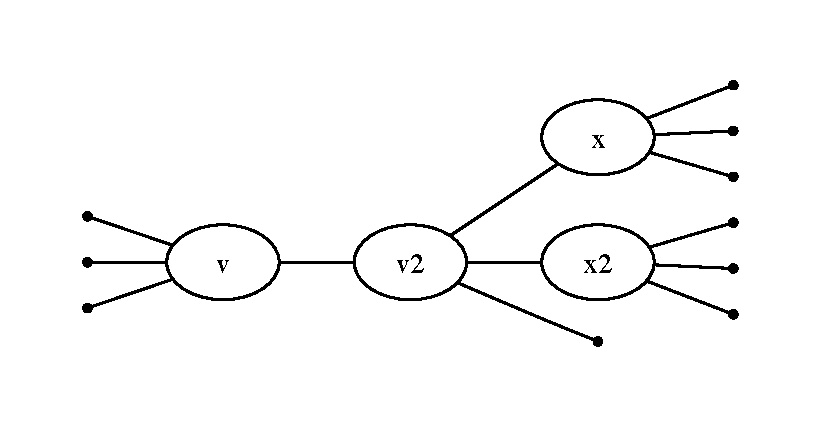
\includegraphics{./images/randomized_matching_delete_edge}
\end{center}
\caption{What edges can be deleted in one round?}
\label{fig:at_least_half}
\end{figure}
\end{pr}

Lemma \ref{lem:at_least_half} alone is not sufficient to prove the logarithmic running time, as the individual stages during the run of the algorithm are not independent\footnote{I think}. We need some more information before we can conclude the bounds on the running time.

\begin{lem} For all $i\geq 1$
\[P(|E_i| \geq 1) \leq |E_1| \cdot 2^{-i+1}\]
\end{lem}

\begin{pr} By Markov's inequality $P(|E_i| \geq 1) \leq \E(|E_i|)$. We want to show that $|E_i|\leq |E_1|\cdot 2^{-i+1}$.

We apply the law of total expectation\footnote{I think that's what it's called} and the previous lemma:

\begin{align*}
\E(|E_i|) &= \sum_{G\subseteq G_1} P(G_{i_1} =G) \cdot \E(|E_i| | G_{i-1}=G)\\
	&=\sum_{G\subseteq G_1}  P(G_{i_1} =G) \cdot \E(|E_{i-1}| -X_{i-1} | G_{i-1}=G)\\
	&=\sum_{G\subseteq G_1}  P(G_{i_1} =G) \cdot (\E(|E_{i-1}| | G_{i-1}=G) - \E( -X_{i-1} | G_{i-1}=G))\\
	&=\sum_{G\subseteq G_1}  P(G_{i_1} =G) \cdot (|E(G)| - \E(X_{i-1} | G_{i-1}=G))\\
	&\stackrel{\text{lem. \ref{lem:at_least_half}}}{=} \sum_{G\subseteq G_1}  P(G_{i_1} =G) \cdot (|E(G)| - \frac{E(G)}{2})\\
	&=\frac 12 \sum_{G\subseteq G_1}  P(G_{i_1} =G) \cdot |E(G)|\\
	&=\frac 12 \E(|E_{i-1}|)\\
\end{align*}

By induction we get the bound claimed in the lemma.
\end{pr}

\begin{lem} Let T be the number of rounds until algorithm \ref{alg:fast_mis} terminates. Then $\E(T) \leq 2\log n+O(1)$\end{lem}

\begin{pr} We have

\begin{align*}
\E(T) &= \sum_{i\geq 1} i P(T=i) \\
	&= \sum_{i\geq 1} P(T\geq i)\\
	&\leq C + \sum_{i> C} P(T\geq i)\\
\intertext{Note that $P\geq i$ implies $|E_i|\geq 1$, otherwise the algorithm would have stopped.}
	&\leq C+ \sum_{i> C} P(|E_i|\geq 1)\\
	&\leq C+ \sum_{i>C} |E_1|\cdot 2^{-i+1}\\
	&\leq C+ n^2 \cdot \sum_{i>C} 2^{-i}\\
	&\leq C+ n^2 \cdot 2\cdot 2^{-C}\\
\end{align*}

Choose $C$ to be $2\log n$ to get the result.
\end{pr}

\paragraph{Remark.} The algorithm may be fast in expectation, but that doesn't guarantee an acceptable running time with high probability. We would like to have a good running time with probability at least $1-n^{-c}$.

\begin{thm} $P(T> c\log n) = O(n^{2-c})$\end{thm}
\begin{pr} $T>i$ implies $E_i\geq 1$, so $P(T > i) \leq |E_1| \cdot 2^{-c\log n} = n^{2-c}$.\end{pr}

\paragraph{Remark.} \begin{enumerate}
\item We don't need to draw real numbers. It is sufficient to communicate $O(\log n)$ bits (exercise). 
\item It's an open problem to beat $O(\log n)$ randomized rounds. There is no known deterministic algorithm that has logarithmic running time.
\end{enumerate}

\subsection{Applications}

\subsubsection{General Graph Colouring}

We already know how to colour graphs of bounded degree in $O(\log^* n)$. We can use algorithm \ref{alg:fast_mis} to colour general graphs in logarithmic time. We construct an auxiliary graph $G^* = (V^*, E^*)$ out of $G$ by doing the following steps

\begin{enumerate}
\item For every $v\in V$ make $d(v)+1$ clones $C_v = \{v_0,v_1,\ldots v_{d(v)}\}$. $V^*$ is the set of all clones.
\item $C_v$ forms a clique in $G^*$
\item If $\{u,v\} \in E$ then $\{u_i,v_i\} \in E^*$ for $0\leq i \leq \min \{d(u),d(v)\}$

\begin{figure}
\begin{center}
\begin{verbatim}
graph G {

	subgraph cluster2 {
		label = "A"
		a -- b
		a -- c
		a -- d
		a -- e
		b -- c
		b -- d
		b -- e
		c -- d
		c -- e
		d -- e
		
	}
	
	subgraph cluster1 {
	  label = "B"
		f -- g
		f -- h
		f -- i
		g -- h
		g -- i
		h -- i
	}
	
	a -- f
	b -- g
	c -- h
	d -- i
}
\end{verbatim}
\end{center}
\end{figure}
\end{enumerate}

\begin{figure}[hbt]
\begin{lstlisting}
simulate Fast-Mis($G^*$) //only local information needed
if $v_i\in $ MIS, then
	$c_v=i$ 
\end{lstlisting}
\caption{An algorithm for general graph colouring}
\label{alg:general_colouring}
\end{figure}

\begin{thm} Algorithm \ref{alg:general_colouring}finds a valid colouring with $\leq \Delta+1$ colours in expected time $O(\log n)$.\end{thm}

\begin{pr} Observations:

\begin{enumerate}
\item Since the clones of a node are in a clique, at most one of them can be in the MIS
\item Let $v\in V$ be any vertex and let $w_1,\ldots,w_d$ be its neighbours in $G$

%picture
Since in the clique are $d+1$ vertices, but it only has $d$ edges to neigbouring cliques, one vertex must be free to join the MIS.

\end{enumerate}

So we get a colouring. We have to show that it's valid, i.e. the indices chosen into the MIS are not equal for neighbouring cliques. But this is obvious, since we have $\{u_i,v_i\}$ edges between cliques.

Since copying the nodes only makes the graph polynomially larger, the logarithmic running time is preserved.
\end{pr}